

  % begin the content of the document
\sloppy  % this to relax whitespacing in favour of straight margins


% title on top of the document
\maintitle{Michelle Swnepoel}{February 1,1994}{Last update on \today}

\nobreakvspace{0.3em}  % add some page break averse vertical spacing

\noindent\href{mailto:michelle4swanepoel.at.gmail.dot.com}{michelle4swanepoel\mbox{}@\mbox{}gmail.com}\sbull
\textsmaller{+}27.836452606\sbull
\\
10 Shamrock Street\sbull
Ferndale Ext 3\sbull
Randburg\sbull

\spacedhrule{0.9em}{-0.4em}  % a horizontal line with some vertical spacing before and after
\begin{center}
\roottitle{Summary}  % a root section title
\end{center}


\vspace{-1.3em}  % some vertical spacing
\begin{multicols}{3}% open a multicolumn environment

\noindent 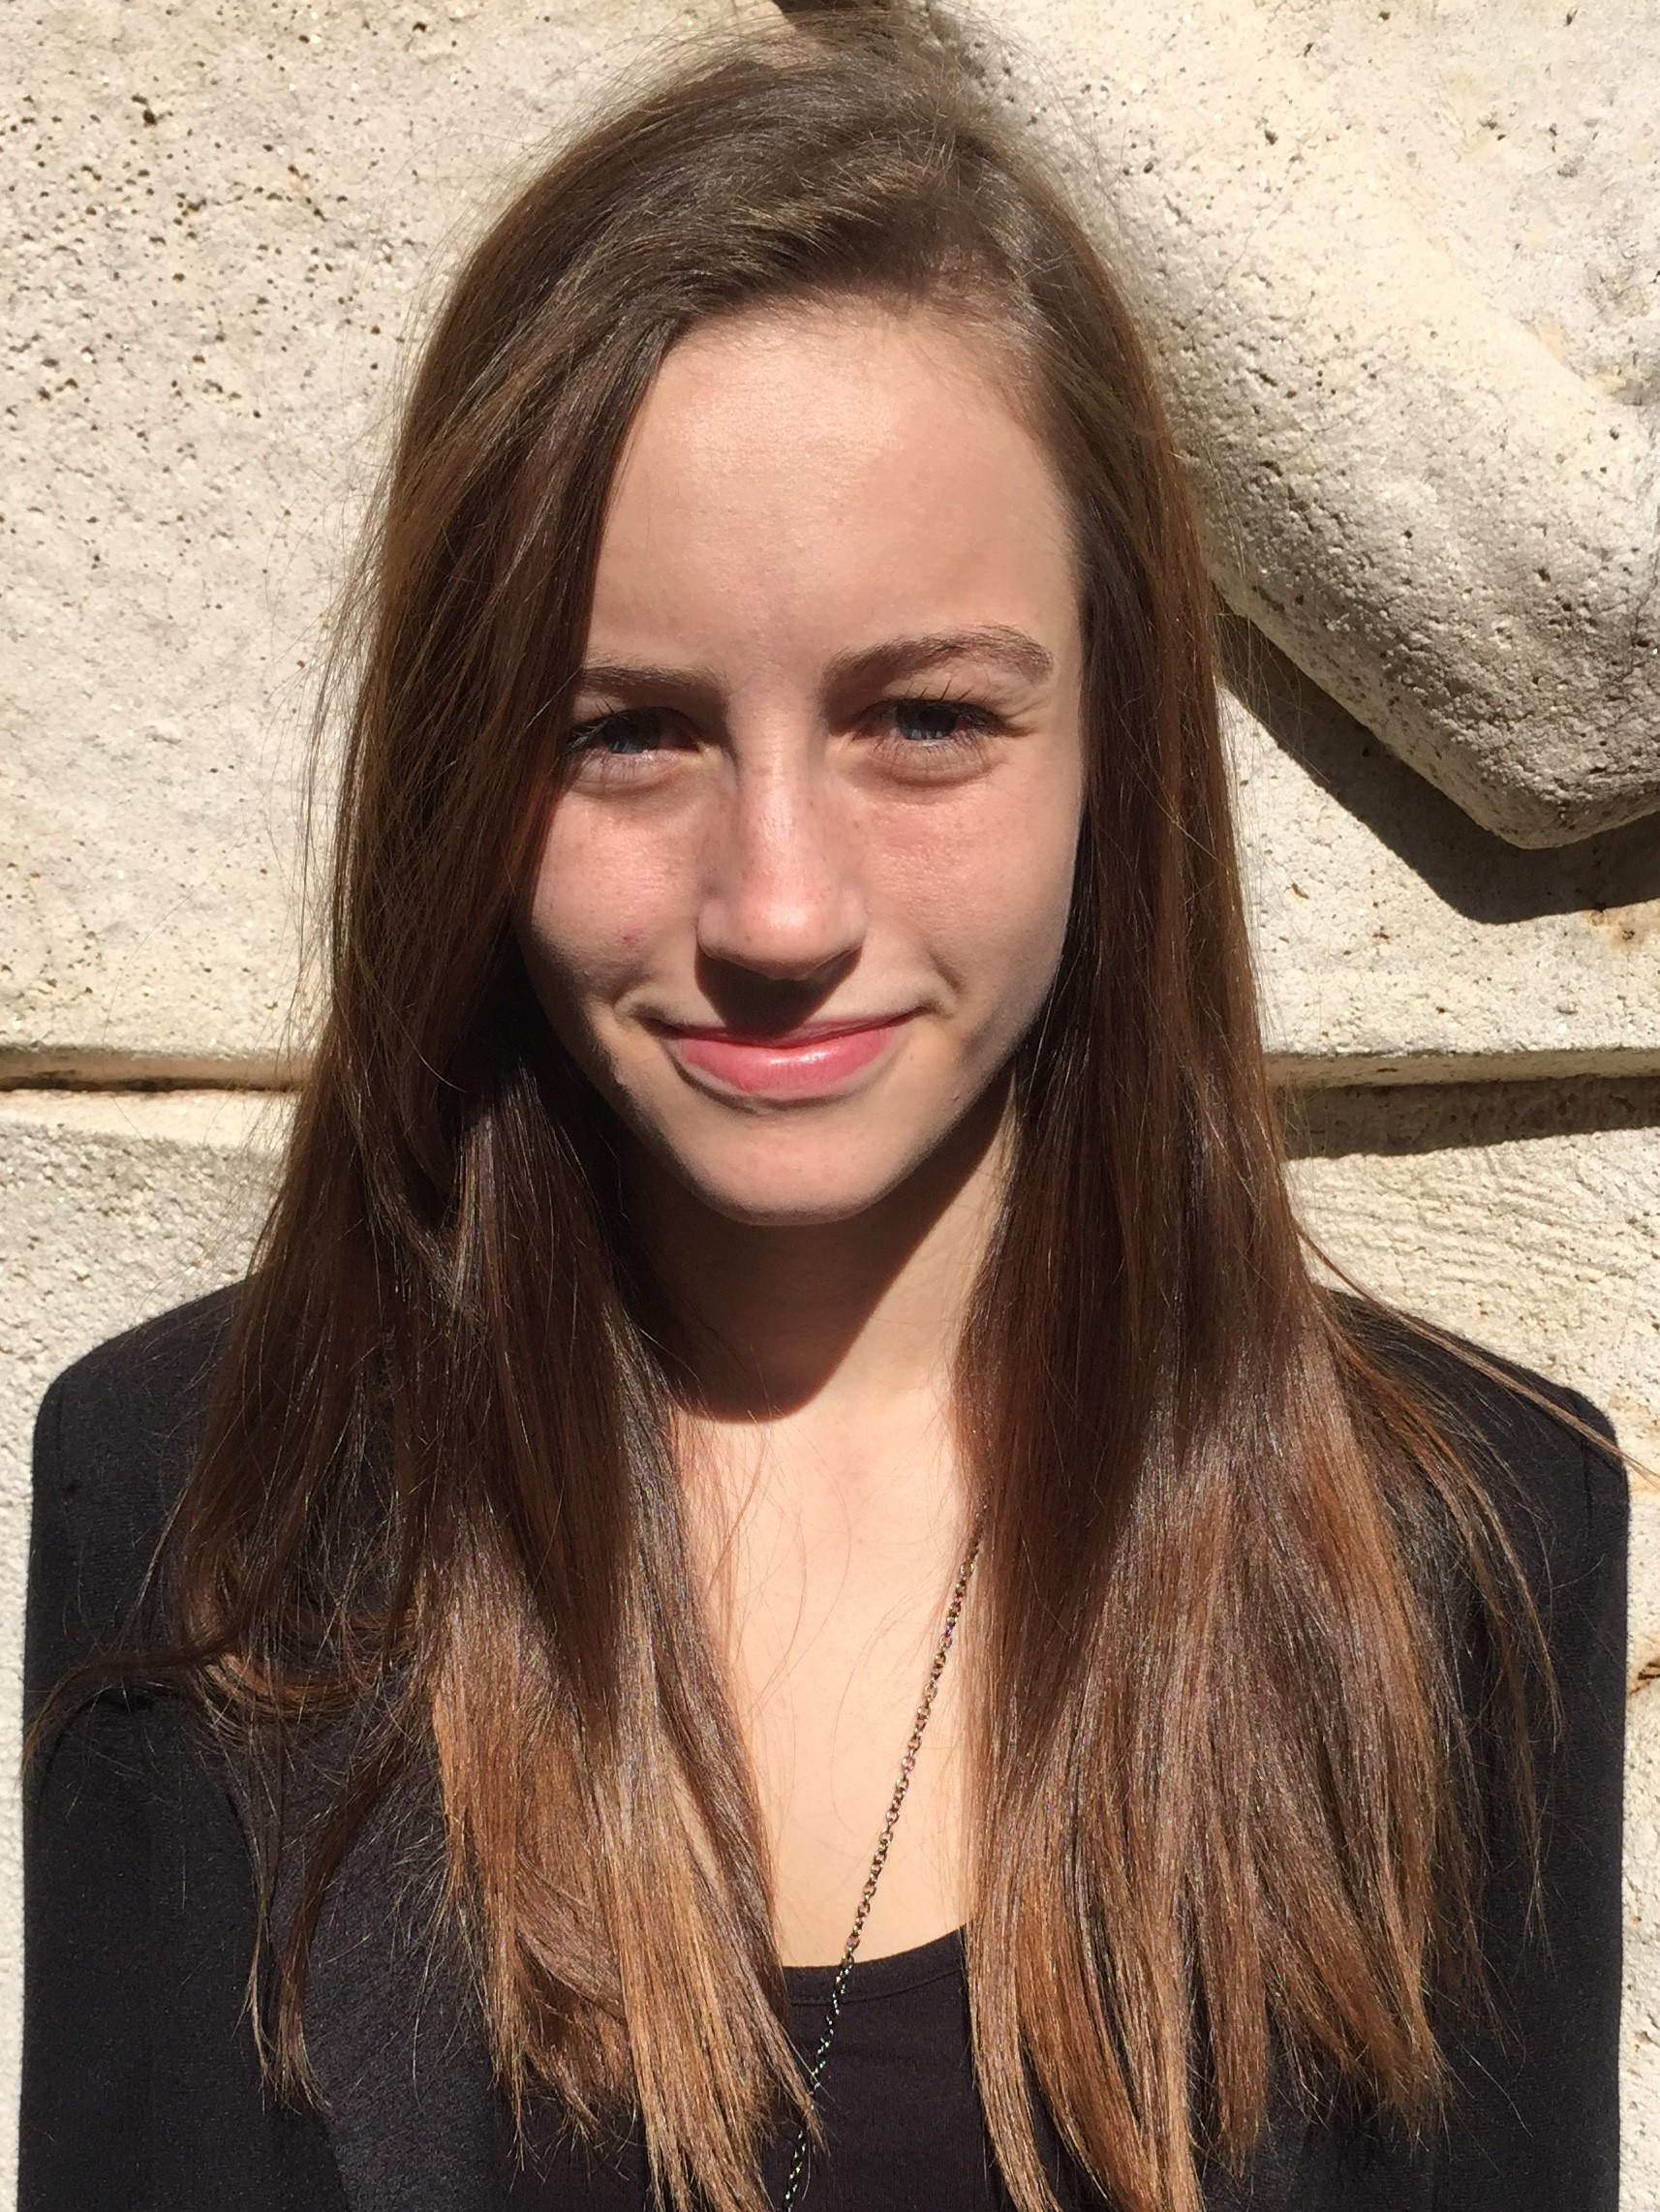
\includegraphics[width=\linewidth]{michelle}\\I see myself as a person who is invested in my personal growth in all aspects of my life. I am currently double majoring and still deciding whether I want to do honours degree next year or start working.  When I feel everything around me is going to fast and that I need a getaway, I will most definitely grab the book I'm currently reading and enjoy a few pages. I also enjoy watching series, building puzzle and playing 30 Seconds with my mom and sister - and always  a cup of coffee. One of my other passions in life is dogs and animals in general. Close friends and family see me as a person who is diligent, respectful, sincere, modest and compassionate. I am an introvert, but enjoy observing and getting to know new people. I get my energy by accomplishing something that I had to work hard for and working with people.


\end{multicols}

\spacedhrule{0em}{-0.4em}

\roottitle{Experience}

    
\headedsection
  {\href{http://www.up.ac.za}{University of Pretoria, Computer Science Department}}
  {\textsc{Hatfield, Pretoria}} {%
  \headedsubsection
    {Teaching Assistant}{Feb\apo14 -- Jul\apo14 and Feb\apo15 -- present}
    {\bodytext{I was a teaching assistant for a Introduction to Computer Science module, where it is needed to understand some
	basic concepts underlying computer science. I am now a teaching assistant for Data Structures and Algorithm, which requires 	the understanding of advanced data structures.\\}}
    }
        
\spacedhrule{-0.2em}{-0.4em}


\roottitle{Technical Skills}

\inlineheadsection  % special section that has an inline header with a 'hanging' paragraph
  {Technical expertise:}
  {Computer Languages: Java, C/C++, assembly, CSS, HTML, JavaScript \(also WebGL\), XML, PHP, AJAX and jQuery}\\

\vspace{0.5em}
\inlineheadsection
  {Natural languages:}
  {Afrikaans \emph{(home language)}, English.}


\spacedhrule{1.6em}{-0.4em}

  
\spacedhrule{1.6em}{-0.4em}  
  
\roottitle{Non - Technical Strengths}

\inlineheadsection
I consider myself as someone with good communications skills, enjoying it to work with people. I will always be open to new experiences and opportunities. Honesty is important to me, thus I will always be be open and trustworthy. I am also someone who grasps a new topic quite quickly. \\

These strengths are propagated throughout my social and professional life.
   
\spacedhrule{1.6em}{-0.4em}  
  
\roottitle{Why DVT Drive Stats?}

\inlineheadsection
  {Because:}
  {When I read the project proposal for the first time, the idea immediately jumped out to me. It sounds like a fun project to do as a team and something we can be proud of afterwards. Even though the project will challenge me and I will have to learn some new technologies and skills, it sounds still within in reach for us as a team to accomplish. }